% ==============================================================================================
\chapter{Dynamic horizontal point load on dam} \label{ch:vibrating_dam_2D}
% ==============================================================================================

% ----------------------------------------------------------------------------------------------
\section{Introduction}
% ----------------------------------------------------------------------------------------------
This benchmark compares the STEM numerical solution against the analytical solution,
for a dynamic horizontal point load on a dam structure with plane-strain conditions.

The analytical solution is presented in~\cite[Chapter~7.3.4]{Kramer_1996}. The analytical solution provides the first
5 natural frequencies of vibration of the dam structure, which are compared against the numerical model.

% ----------------------------------------------------------------------------------------------
\section{Model Description}
% ----------------------------------------------------------------------------------------------

% ..............................................................................................
\subsection{Geometry, mesh and loading}
% ..............................................................................................
The reference geometry as presented in~\cite{Kramer_1996} is given with feet units. For consistency with the rest of
the benchmarks in this report, the geometry has been converted to SI units (meters).

The soil domain is modelled in 2D and represents a triangle with base \qty{160.02}{\meter} and height \qty{45.72}{\meter},
the left slope is inclined with a ratio of 2:1 (horizontal to vertical), while the right slope is inclined with a ratio
of 1.5:1. The mesh is created with higher order elements and uses an average element size of \qty{2}{\meter}.
Figure~\ref{fig:vibrating_dam_mesh} illustrates the geometry and mesh adopted for the analysis.

The horizontal point load with a magnitude of \qty{1e6}{\newton\per\meter} is instantly applied at the top of the dam
structure and is kept constant during the analysed time window.

The nodes at the bottom are fully fixed, while the rest of the nodes within the whole surface can only move in the
x-direction.

\begin{figure}
    \centering
    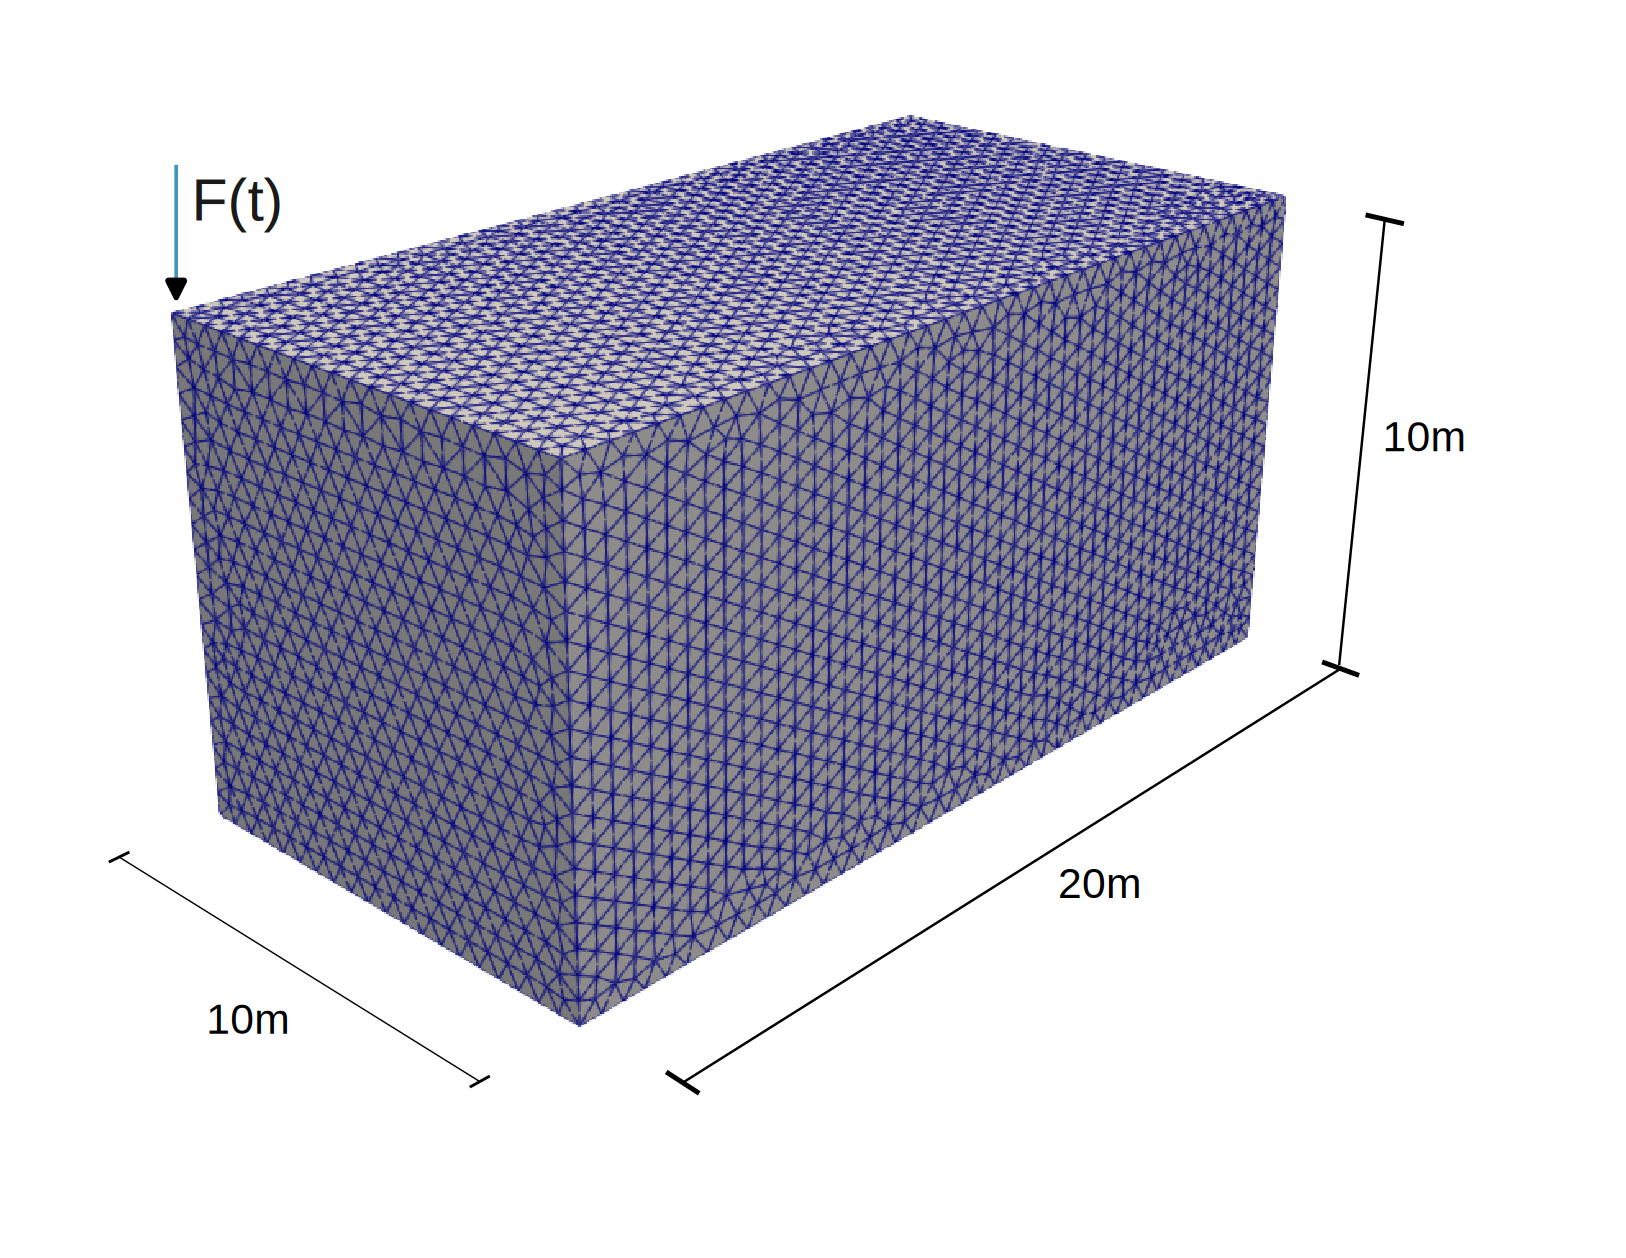
\includegraphics[width=0.75\textwidth]{vibrating_dam/mesh.png}
    \caption{Geometry, mesh and boundary conditions adopted for the vibrating dam benchmark.}
    \label{fig:vibrating_dam_mesh}
\end{figure}

% ..............................................................................................
\subsection{Materials and numerical parameters}
% ..............................................................................................
The soil is modelled as an one-phase continuum with a linear elastic constitutive law, with the
following parameters:

\begin{itemize}[noitemsep,topsep=0pt,parsep=0pt,partopsep=0pt]
    \item Young's modulus: \qty{722}{\mega\pascal},
    \item Poisson ratio: 0.49,
    \item Density: \qty{2000}{\kilogram\per\meter\cubed}.
\end{itemize}

Material damping is excluded from this analysis.

The dynamic analysis is performed over a \qty{2}{\second} time window, with a time step of \qty{0.001}{\second}.
The system of equations is solved using the Newmark time integration~\cite{Newmark_1959} scheme with
parameters $\beta = 0.25$ and $\gamma = 0.5$.

% ----------------------------------------------------------------------------------------------
\section{Results}
% ----------------------------------------------------------------------------------------------
Figure~\ref{fig:vibrating_dam_results} presents the power spectral density of the horizontal displacement of the
 top of the dam.
The figure compares the STEM results against the analytical solution.
If follows that the peaks of the power spectral density plot occur at exactly the expected first 5 natural frequencies,
demonstrating the accuracy of the STEM for this type of dynamic loading condition.

\begin{figure}[h]
    \centering
    \includegraphics[width=0.8\textwidth]{vibrating_dam/power_spectral_density.pdf}
    \caption{Power spectral density plot of the horizontal displacement at the top of the dam}
    \label{fig:vibrating_dam_results}
\end{figure}
